\chapter{Vision: Learning from Images}
\label{ch:vision}

Vision models are difficult not because images are large arrays of numbers, but because the same object can appear under different lighting, scales, viewpoints, backgrounds, and occlusions. A useful visual representation must preserve what matters and ignore what should not change the answer. This chapter studies vision from that modeling perspective. We begin with task formulation, since classification, detection, and segmentation each demand different outputs. We then work through convolution, pooling, augmentation, transfer, and robustness as ways to control which visual variation counts as signal and which counts as nuisance. The running question is not whether a model recognizes an object, but whether it learned the right cue under the conditions the deployment camera will actually produce. \emph{Deployment-camera realism} means matching the data, stress tests, and failure review to the actual lens, mounting position, and acquisition conditions of the deployed system. The chapter later treats \emph{saliency} maps---visual overlays showing which image regions most affected a prediction---as diagnostic evidence rather than proof. By the end, you should be able to diagnose a vision problem in terms of invariance, structure, and deployment realism rather than architecture alone.

\section{Opening Dilemma: The Same Object Can Look Like Many Different Pixel Arrays}

Suppose the task is to support a road-scene system that must detect pedestrians. The same person on the roadside can appear under bright sun, at dusk, under headlight glare, partially occluded, seen from different camera heights, or blurred by motion. The semantic object stays the same, but the pixel array changes drastically.

Vision therefore should not begin with architecture names. It should begin with a judgment question: which variations should preserve the label, and which should change it? A pedestrian shifted slightly within the image is still a pedestrian. A change in lighting should usually not erase the label. But removing the pedestrian entirely, swapping the person for a traffic sign, or switching from detection to segmentation should all change what the model outputs.

Keep one running case in view throughout this chapter: a dashboard-camera pedestrian detector for a low-speed campus shuttle. The detector must work through windshield glare, dusk and night conditions, light rain, partial occlusion, and camera-specific geometry. This single case forces the chapter to connect invariance, architecture, augmentation, shortcuts, and deployment-camera realism inside one visual system rather than treating them as separate ideas.

That dilemma sets the chapter's shape. First we fix the output object and the invariance audit. Then we clarify annotation and locality. Next we turn to augmentation and transfer. Finally we ask how to distrust benchmark success correctly.

\section{Problem-Solving Technique: Invariance Audit}

Before training a vision model, write down which variations should preserve the label, which should change it, which sensor or camera changes are realistic in deployment, and what spatial detail the downstream task actually needs.

This is the chapter's most reusable habit. The audit connects task formulation, augmentation, architecture, and evaluation. Image classification may need broad invariance to small translations and lighting changes. Segmentation may tolerate that same variation while demanding far more spatial detail. If deployment uses a different camera than the training set, the camera itself becomes part of the modeling problem.

\begin{figure}[t]
\centering
\resizebox{\linewidth}{!}{\definecolor{auditcolor}{rgb}{0.15,0.35,0.75}
\definecolor{taskcolor}{rgb}{0.75,0.25,0.15}
\definecolor{modelcolor}{rgb}{0.20,0.60,0.20}
\definecolor{evalcolor}{rgb}{0.60,0.15,0.65}

\begin{tikzpicture}[
    x=1cm, y=1cm,
    font=\small,
    %% Shared box styles – 3.2cm wide, 4.5cm column spacing
    pbox/.style={draw, rounded corners=3pt,
                 minimum width=3.2cm, minimum height=1.10cm,
                 align=center, font=\small},
    audit/.style={pbox, fill=auditcolor!15, draw=auditcolor},
    task/.style ={pbox, fill=taskcolor!15,  draw=taskcolor},
    model/.style={pbox, fill=modelcolor!15, draw=modelcolor},
    eval/.style ={pbox, fill=evalcolor!15,  draw=evalcolor},
    %% Annotation note style – centred so text stays within column
    note/.style={align=left, font=\footnotesize, text width=3.0cm},
    arr/.style={-{Stealth[length=3mm]}, thick},
    fbk/.style={-{Stealth[length=2.5mm]}, dashed, gray!70, thick},
]

%% ── Column x-centres: 4.5 cm apart ──────────────────────────────────────
%%    audit=1.6   task=6.1   model=10.6   eval=15.1
%% ── Row y-centres ────────────────────────────────────────────────────────
%%    phase=10.5  input=9.4  row1=7.85  row2=6.05  robustness=4.2  notes=2.3

%% ── Phase labels ──────────────────────────────────────────────────────────
\node[font=\footnotesize\bfseries, auditcolor] at ( 1.6,10.5) {DESIGN};
\node[font=\footnotesize\bfseries, taskcolor]  at ( 6.1,10.5) {SPECIFICATION};
\node[font=\footnotesize\bfseries, modelcolor] at (10.6,10.5) {IMPLEMENTATION};
\node[font=\footnotesize\bfseries, evalcolor]  at (15.1,10.5) {VALIDATION};

%% ── Input node ──────────────────────────────────────────────────────────
\node[pbox, fill=gray!12, draw=gray!60] (input) at (1.6,9.4)
    {Raw image\\dashboard camera};

%% ── Row 1 boxes ──────────────────────────────────────────────────────────
\node[audit] (inv)  at ( 1.6,7.85) {Invariance\\audit};
\node[task]  (tdef) at ( 6.1,7.85) {Task\\formulation};
\node[model] (arch) at (10.6,7.85) {Architecture\\choice};
\node[eval]  (evl)  at (15.1,7.85) {Evaluation\\strategy};

%% ── Row 2 boxes ──────────────────────────────────────────────────────────
\node[audit] (nui)  at ( 1.6,6.05) {Nuisance vs.\\signal};
\node[task]  (out)  at ( 6.1,6.05) {Output\\structure};
\node[model] (aug)  at (10.6,6.05) {Augmentation\\policy};
\node[eval]  (str)  at (15.1,6.05) {Stress\\testing};

%% ── Main horizontal arrows (row 1) ───────────────────────────────────────
\draw[arr] (input) -- (inv);
\draw[arr] (inv.east)  -- (tdef.west);
\draw[arr] (tdef.east) -- (arch.west);
\draw[arr] (arch.east) -- (evl.west);

%% ── Vertical connections ──────────────────────────────────────────────────
\draw[arr] (inv.south)  -- (nui.north);
\draw[arr] (tdef.south) -- (out.north);
\draw[arr] (arch.south) -- (aug.north);
\draw[arr] (evl.south)  -- (str.north);

%% ── Robustness box: sits directly below row 2, above the notes ───────────
\node[draw=evalcolor, rounded corners=4pt, fill=evalcolor!8, align=center,
      minimum width=15.5cm, minimum height=1.10cm, font=\small] (rob) at (8.35,4.2)
    {\textbf{Shortcut Learning \& Robustness Analysis}\\[2pt]
     \footnotesize Background cues \ $\cdot$\ Camera artefacts
     \ $\cdot$\ Crossing paint \ $\cdot$\ Annotation bias};

%% ── Connections to robustness box (short, clear descent) ────────────────
\draw[arr] (out.south) to[out=270,in=120] (rob.north west);
\draw[arr] (aug.south) to[out=270,in=90]  (rob.north);
\draw[arr] (str.south) to[out=270,in=60]  (rob.north east);

%% ── Feedback loops ───────────────────────────────────────────────────────
\draw[fbk] (rob.west) to[out=180,in=270] (nui.south);
\draw[fbk] (str.south east) to[out=315,in=0] (aug.east);

%% ── Annotation notes: below robustness box, out of arrow paths ───────────
\node[note, auditcolor] at (1.6,2.3)
    {\textbf{Ignore:}\\
     small translations,\\
     lighting shifts,\\
     mild blur};

\node[note, taskcolor] at (6.1,2.3)
    {\textbf{Output:}\\
     classification,\\
     detection with boxes,\\
     or segmentation};

\node[note, modelcolor] at (10.6,2.3)
    {\textbf{Valid transforms:}\\
     spatial crops,\\
     color jitter,\\
     weather noise};

\node[note, evalcolor] at (15.1,2.3)
    {\textbf{Critical slices:}\\
     night conditions,\\
     new cameras,\\
     edge cases};

\end{tikzpicture}
}
\caption{The vision development pipeline integrates invariance auditing, task formulation, architecture choices, and evaluation strategy into a coherent workflow. Each stage blocks different failure modes, with feedback loops revealing shortcut learning and robustness gaps that require pipeline redesign.}
\label{fig:vision-pipeline}
\end{figure}

You cannot interpret vision performance before the invariance audit is clear. A model cannot be said to work unless we know what it was supposed to ignore, what it was supposed to preserve, and what the deployment camera will actually produce. A useful workflow runs in this order: start from the task and required output, run the invariance audit, make the annotation policy explicit, pick the smallest baseline that matches the output shape, add augmentations only for label-preserving variation, then compare training from scratch against a frozen pretrained backbone and a fine-tuned pretrained backbone on deployment-relevant slices. The running artifact is a vision design and stress-test card with fields for task type, intended signal, nuisance variation, deployment camera, likely shortcut risks, and the slices or stress tests that would reveal failure before deployment.

\section{Task Formulation Before Architecture Depth}

One of the biggest mistakes in vision is asking ``CNN or transformer?'' before asking what output is actually required. This section settles what the system must produce, and therefore what evidence later architecture and evaluation must preserve.

\subsection{Classification}

Classification asks what is in the image. A road-scene classifier might answer ``pedestrian present'' or ``no pedestrian present.'' This is useful but rarely sufficient for safety-critical settings.

On the same scene, classification answers a coarse yes/no question about the whole image. It does not say where the pedestrian is, whether the object is partially occluded, or whether the model confused the crossing with the person. The output object must therefore be chosen before architecture depth becomes the main topic.

\subsection{Detection}

Object detection asks both \emph{what} appears and \emph{where}. A detector must localize relevant objects, usually with bounding boxes, and assign categories.

\begin{mathlens}
Suppose a predicted bounding box is \(B\) and the ground-truth box is \(G\). A standard overlap score is intersection over union:
\[
\mathrm{IoU}(B,G)=\frac{|B\cap G|}{|B\cup G|}.
\]
If the class is correct and IoU exceeds a chosen threshold such as \(0.5\), the detection is often counted as a hit. IoU matters because detection is not only about naming an object; it is about placing the box tightly enough that the localization is operationally useful.
\end{mathlens}

\begin{practicalnote}
A detector usually makes three linked predictions at many candidate locations or regions: is there an object here, what class is it, and how should the current box move to fit it better? Detection errors therefore come in three distinct forms: missed candidates, mislabeled objects, and badly placed boxes.
\end{practicalnote}

\subsection{Segmentation}

Segmentation assigns labels to pixels or regions rather than to the whole image. Semantic segmentation marks categories such as road, pedestrian, and sky. Instance segmentation goes further and separates individual object instances.

\begin{mathlens}
If \(M\) is the predicted mask and \(G\) the ground-truth mask, two common overlap scores are
\[
\begin{aligned}
\mathrm{IoU}(M,G) &= \frac{|M\cap G|}{|M\cup G|}, \\
\mathrm{Dice}(M,G) &= \frac{2|M\cap G|}{|M|+|G|}.
\end{aligned}
\]
Both reward overlap, and for a fixed pair of masks Dice is a monotone transform of IoU. Practitioners often report both because small foreground regions can make either score swing sharply under modest boundary errors.
\end{mathlens}

\begin{example}[Why Small Masks Are Hard]
Missing twenty pixels on a large road region barely changes the score. Missing twenty pixels on a pedestrian silhouette can erase an arm or leg. Segmentation metrics must therefore be read together with class size and boundary importance, not as if every pixel error carried the same operational weight.
\end{example}

\subsection{Tracking and Other Structured Vision Tasks}

Other vision tasks include pose estimation, keypoint detection, tracking across video frames, depth estimation, and optical flow. Vision is not one problem but a family of problems organized around spatial perception.

For video, a single-frame detector may suffice if each frame is evaluated independently. Tracking or temporal smoothing enters the task the moment the system must follow the same object over time.

\subsection{Why Structured Outputs Need Structured Evaluation}

The output type changes the evidence you must collect. Classification can usually be judged with image-level accuracy, precision, recall, and calibration. Detection needs those same habits plus localization quality, because a box in the wrong place is not the same failure as a box with the wrong class. Segmentation needs overlap metrics and boundary checks because the task is about regions rather than whole images. Tracking adds temporal consistency because the system must keep identity stable across frames. In each case, evaluation should match the output object, not only the underlying image.

\begin{practicalnote}
Structured outputs create structured failures. Classification can be wrong about an object's presence; detection can be wrong about presence or placement; segmentation can be wrong about boundaries or small regions; tracking can be wrong about identity over time. The model choice should make those failure modes legible.
\end{practicalnote}

\begin{decisionbox}
\textbf{Choose the output before the backbone.} Use classification when only image-level presence or absence matters, detection when location or count matters, segmentation when region shape or fine boundary support matters, and tracking when identity has to remain stable over time rather than only within one frame.
\end{decisionbox}

Figure~\ref{fig:vision-street-scene} makes this concrete. A single street image can support several outputs depending on what the downstream system needs.

\begin{figure}[t]
\centering
\definecolor{c8road}{RGB}{130,130,130}
\definecolor{c8side}{RGB}{210,200,185}
\definecolor{c8cls}{RGB}{56,103,170}
\definecolor{c8det}{RGB}{180,40,40}
\definecolor{c8seg1}{RGB}{100,160,100}
\definecolor{c8seg2}{RGB}{220,233,251}
\definecolor{c8seg3}{RGB}{240,220,180}
\definecolor{c8ped}{RGB}{214,120,62}
\resizebox{\linewidth}{!}{%
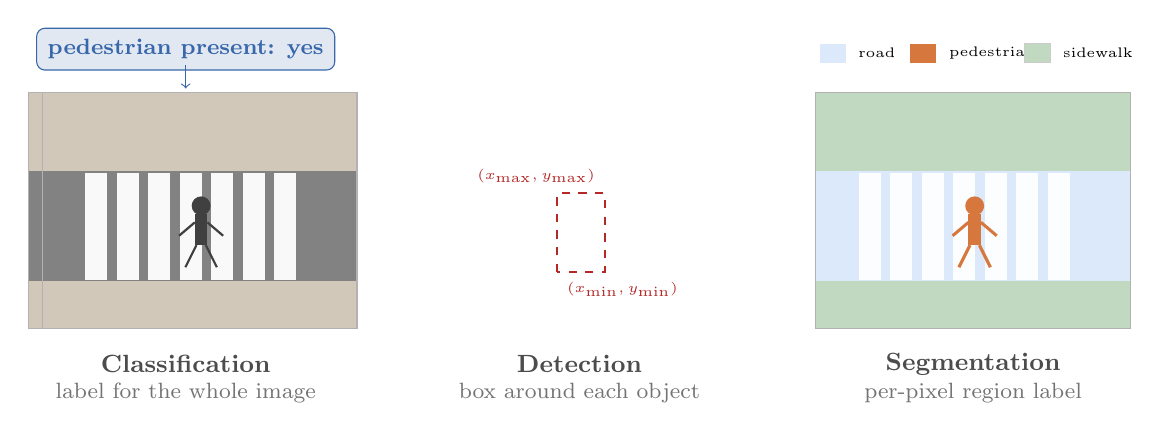
\begin{tikzpicture}[x=1cm, y=1cm, font=\small]

%% ── Macro: draw a bird's-eye road scene at xshift ───────────────────────
%% Scene: 4cm wide × 3cm tall with one pedestrian in the shuttle camera view.
\newcommand{\roadscene}[1]{%  #1 = xshift value
  \begin{scope}[xshift=#1]
    %% sidewalk top
    \fill[c8side]  (0,2.0) rectangle (4.0, 3.0);
    %% road
    \fill[c8road]  (0,0.6) rectangle (4.0, 2.0);
    %% crosswalk stripes (white)
    \foreach \s in {0.55,0.95,1.35,1.75,2.15,2.55,2.95} {
      \fill[white!95!c8road] (\s,0.62) rectangle (\s+0.28,1.98);
    }
    %% sidewalk bottom
    \fill[c8side]  (0,0.0) rectangle (4.0, 0.6);
    %% pedestrian silhouette
    \fill[black!75] (2.02,1.56) circle (0.12);
    \fill[black!75] (1.94,1.06) rectangle (2.10,1.46);
    \draw[black!75, line width=0.8pt] (1.94,1.35) -- (1.74,1.18);
    \draw[black!75, line width=0.8pt] (2.10,1.35) -- (2.30,1.18);
    \draw[black!75, line width=0.8pt] (1.96,1.06) -- (1.82,0.78);
    \draw[black!75, line width=0.8pt] (2.08,1.06) -- (2.22,0.78);
    %% thin border
    \draw[black!30, thin] (0,0) rectangle (4.0,3.0);
  \end{scope}%
}

%% ── Panel spacing ────────────────────────────────────────────────────────
%%    panels at x = 0, 5.0, 10.0  (4cm wide + 1cm gap)

%% ─── Panel 1 : Classification ────────────────────────────────────────────
\roadscene{0}
%% label badge
\node[fill=c8cls!15, draw=c8cls, rounded corners=3pt,
      font=\footnotesize\bfseries, text=c8cls, inner sep=4pt]
  at (2.0, 3.55) {pedestrian present: \textbf{yes}};
\draw[->, thin, c8cls] (2.0, 3.35) -- (2.0, 3.05);
\node[font=\small\bfseries, black!70] at (2.0,-0.45) {Classification};
\node[font=\footnotesize, black!55]   at (2.0,-0.82) {label for the whole image};

%% ─── Panel 2 : Detection ─────────────────────────────────────────────────
\roadscene{5.0}
%% bounding box around the pedestrian
\draw[c8det, thick, dashed] (6.72, 0.72) rectangle (7.32, 1.72);
%% corner coordinates
\node[font=\tiny, c8det, anchor=north west] at (6.72, 0.72)
  {$(x_{\min},y_{\min})$};
\node[font=\tiny, c8det, anchor=south east] at (7.32, 1.72)
  {$(x_{\max},y_{\max})$};
\node[font=\small\bfseries, black!70] at (7.0,-0.45) {Detection};
\node[font=\footnotesize, black!55]   at (7.0,-0.82) {box around each object};

%% ─── Panel 3 : Segmentation ──────────────────────────────────────────────
%% Re-draw the scene with colour-coded regions
\begin{scope}[xshift=10.0cm]
  %% sidewalk top - green
  \fill[c8seg1!40] (0,2.0) rectangle (4.0,3.0);
  %% road - blue-ish
  \fill[c8seg2]    (0,0.6) rectangle (4.0,2.0);
  %% crosswalk stripes remain part of the road surface
  \foreach \s in {0.55,0.95,1.35,1.75,2.15,2.55,2.95} {
    \fill[white!92!c8seg2] (\s,0.62) rectangle (\s+0.28,1.98);
  }
  %% sidewalk bottom - green
  \fill[c8seg1!40] (0,0.0) rectangle (4.0,0.6);
  %% pedestrian mask
  \fill[c8ped] (2.02,1.56) circle (0.12);
  \fill[c8ped] (1.94,1.06) rectangle (2.10,1.46);
  \draw[c8ped, line width=1.1pt] (1.94,1.35) -- (1.74,1.18);
  \draw[c8ped, line width=1.1pt] (2.10,1.35) -- (2.30,1.18);
  \draw[c8ped, line width=1.1pt] (1.96,1.06) -- (1.82,0.78);
  \draw[c8ped, line width=1.1pt] (2.08,1.06) -- (2.22,0.78);
  \draw[black!30, thin] (0,0) rectangle (4.0,3.0);
  %% legend chips – spaced so labels don't clip
  \fill[c8seg2]    (0.05, 3.38) rectangle (0.38, 3.62);
  \node[font=\tiny, anchor=west] at (0.42, 3.50) {road};
  \fill[c8ped]     (1.20, 3.38) rectangle (1.53, 3.62);
  \node[font=\tiny, anchor=west] at (1.57, 3.50) {pedestrian};
  \fill[c8seg1!40] (2.65, 3.38) rectangle (2.98, 3.62);
  \draw[black!20, thin] (2.65, 3.38) rectangle (2.98, 3.62);
  \node[font=\tiny, anchor=west] at (3.02, 3.50) {sidewalk};
\end{scope}
\node[font=\small\bfseries, black!70] at (12.0,-0.45) {Segmentation};
\node[font=\footnotesize, black!55]   at (12.0,-0.82) {per-pixel region label};

\end{tikzpicture}%
}
\caption{The same dashboard-camera frame can be read three ways depending on the output required. Classification asks whether a pedestrian is present anywhere in the frame. Detection localizes the pedestrian with a bounding box. Segmentation assigns labels at pixel level, including the pedestrian mask. Task formulation must come first because each output demands a different loss, metric, and architecture head.}
\label{fig:vision-street-scene}
\end{figure}

\begin{table}[t]
\centering
\small
\begin{tabular}{p{2.12cm}p{7.83cm}}
\toprule
Task & Output on the same road-scene image \\
\midrule
Classification & \texttt{pedestrian present = yes} \\
Detection & \texttt{pedestrian = [x\_min, y\_min, x\_max, y\_max]} \\
Segmentation & Pixelwise mask separating pedestrian, road, sidewalk, and background \\
\bottomrule
\end{tabular}
\caption{The same image can define very different output structures. This is why task formulation must come before architecture choice.}
\label{tab:vision-task-output-structure}
\end{table}

\begin{example}[Why Task Formulation Matters]
A system that classifies a dashboard-camera frame as ``contains a pedestrian'' is not enough for the campus shuttle. The shuttle still needs to localize the person, distinguish them from nearby background structure, and preserve enough spatial detail to support downstream decisions. Decide the output requirement before architecture depth becomes the main topic.
\end{example}

\begin{practicalnote}
Model choice follows the output object. Image-level labels suggest a classification head and image-level evaluation. Box labels suggest a detector with localization-aware evaluation. Pixel masks suggest a segmentation head with overlap and boundary checks. When the failure pattern is wrong, the next question is usually whether the annotation policy or output type was underframed---not whether the network was too small.
\end{practicalnote}

\begin{thinkingtool}
\textbf{Task-specific evaluation.} Judge classification with accuracy, precision, recall, and calibration if the output drives a decision. Detection must also respect localization, so IoU and false positives matter alongside class recall. Segmentation usually needs overlap quality such as IoU or Dice, plus boundary behavior when fine spatial detail matters.
\end{thinkingtool}

\subsection{A Running Case: What the Camera Actually Sees}

Suppose the campus shuttle uses a forward-facing dashboard camera mounted low behind the windshield. For the rest of this chapter, treat the real task as \emph{pedestrian detection}, not scene classification, because the system must know where the person is---not only whether one is somewhere in the frame. This running case anchors the rest of the chapter: annotation policy, locality assumptions, augmentation choices, shortcut hypotheses, and deployment slices all answer to the same detector.

The camera is not neutral. A low-mounted dashboard camera sees glare from the glass, reflections from the dashboard, raindrops and smear marks on the windshield, seasonal shadows, and strong scale changes as pedestrians move from far away to very close. A benchmark image can therefore look visually clean while still being a weak proxy for deployment. The invariance audit is already doing work here: small horizontal shifts, mild lighting changes, and modest blur should usually preserve the label, while heavy occlusion, extreme darkness, or viewpoint changes that make the person unresolvable may change what the system can reliably output.

\begin{practicalnote}
In vision, the image is not the world. It is the output of a camera, lens, mounting position, exposure system, and environment. A good vision practitioner keeps asking what that acquisition process adds or removes before the model ever sees the scene.
\end{practicalnote}

\begin{warningbox}
For image sequences or camera data, avoid random splits that put near-duplicate frames on both sides of the evaluation boundary. Split by camera, route, day, clip, or location when those sources could leak the same visual context into train and test.
\end{warningbox}

\section{Annotation Ontology and Label Ambiguity}

Once the output object is fixed, the next question is what the labels actually mean. Every vision dataset rests on an annotation policy that defines---sometimes implicitly---which objects count, what counts as an occurrence, and how annotators should resolve ambiguous cases. That policy is a modeling decision. It shapes the label space, and therefore the task, before any image reaches any model.

\paragraph{Object boundary ambiguity.}
For the pedestrian-detector running case, the annotation policy must decide whether to count a person seen through a store window, behind a fence, with only a headless torso visible at the image boundary, or with their back turned. Different policies on these questions produce different label sets. A model trained under one policy can behave very differently from a model trained under another, even on the same raw images.

\paragraph{Scale and minimum-size conventions.}
Objects at long range are often tiny in the image. Below some pixel area, even a human annotator cannot resolve the object reliably. Detection datasets therefore often define a minimum bounding-box area for inclusion. That threshold is a property of the annotation protocol, not of reality. A model trained with a $32 \times 32$ pixel minimum was never taught to find smaller objects, which is not the same as saying the deployment system is allowed to miss them.

\paragraph{Annotator disagreement.}
When two annotators draw different bounding boxes around the same pedestrian, or one annotator marks an occluded person and another does not, the disagreement usually reflects genuine ambiguity rather than careless labeling. The annotation protocol must resolve this ambiguity with explicit rules. Explicit rules do not eliminate the underlying fuzziness; they replace it with a conventionalized definition that some downstream uses will satisfy and others will not.

\begin{example}[Annotation Policy Shapes Recall]
Suppose a pedestrian-detector dataset uses a policy that excludes heavily occluded people (visible fraction below 30\%). A model trained on this dataset learns to suppress predictions on heavily occluded cases. In a safety evaluation, engineers later discover that the model misses pedestrians partially hidden behind parked vehicles. The model is behaving correctly under its training policy. The training policy was wrong for the deployment context.
\end{example}

\begin{thinkingtool}
\textbf{Label space audit.} Before training a vision model, write down the annotation rules that govern edge cases: minimum object size, occlusion policy, boundary handling, and multiple-instance rules. Then ask whether those rules are defensible for the deployment context. The label space is a modeling choice, not a given.
\end{thinkingtool}

With the output object and annotation policy fixed, the next question is representational: what local visual structure must the model detect reliably across the image?

\section{Why Raw Pixels Are Not Enough}

Images are often described as arrays of pixels, but that description is too weak to explain why vision is difficult. A photograph is not merely a grid of numbers; it is the joint result of lighting, geometry, occlusion, texture, viewpoint, scale, and sensor properties. Different pixel arrays can represent the same object, and nearly identical arrays can represent different scenes.

This is the core educational point. Vision is hard because raw measurements do not come with meaning attached. A model must infer edges, parts, shapes, textures, and object relationships from those measurements. The real challenge is building internal descriptions that remain useful under translation, clutter, lighting change, background change, and viewpoint variation.

Classical computer vision relied heavily on hand-designed features: edges, corners, texture histograms, local descriptors, and shape cues. Those pipelines remain conceptually important because they show what practitioners once thought stable visual structure looked like. Deep learning changed the field not by making structure irrelevant, but by making feature extraction itself learnable. The next section gives the chapter's first architectural answer: ask the same local question across the image rather than treating every pixel position as unrelated.

\section{Convolution as a Repeated Local Question}

\begin{practicalnote}
\textbf{Reading order.} If convolution is new, read the vertical-edge worked example first and then return to the theorem language about equivariance. The example supplies the visual intuition; the theorem names the general property that the example suggests.
\end{practicalnote}

\begin{definition}[Convolutional Layer]
A convolutional layer applies a small learnable filter across an image, producing a feature map whose values measure how strongly the filter matches local patterns at each position.
\end{definition}

The right headline for convolution is simple. It is also the first concrete architectural response to the invariance audit:

\begin{center}
\emph{Convolution matters because vision is local before it is global.}
\end{center}

Two related terms help before the notation. A representation is \emph{equivariant} when an input change produces a corresponding, structured change in the representation---for example, a feature map that shifts along with a shifted image. A decision rule is closer to \emph{invariant} when the answer stays effectively the same under small label-preserving changes. Vision systems usually want equivariant intermediate features and more invariant final outputs.

Suppose an image is represented by a grid $X$ and a small filter $K$ by a $3 \times 3$ matrix. Using the standard deep-learning convention, the local filtering response at location $(i,j)$ is
\[
S_{i,j} = \sum_{u=0}^{2}\sum_{v=0}^{2} K_{u,v} X_{i+u,j+v}.
\]
The filter slides across the image and produces a new grid of responses. One filter may respond to horizontal edges, another to vertical edges, another to corners; later filters can respond to more complex motifs built from earlier ones.
This operation is technically cross-correlation rather than flipped-kernel convolution, but deep-learning libraries call it convolution. The theorem below uses the unflipped filtering operator defined by the displayed sum.

\begin{practicalnote}
For the pedestrian-detector running case, these feature maps are not the final output. They are local evidence maps. A detector turns such evidence into objectness scores, class scores, and bounding boxes, then evaluates localization with IoU and detection precision/recall. A toy digit classifier teaches convolution and pooling, but the deployment task also needs box geometry and false-positive control.
\end{practicalnote}

\begin{prereqbridge}
The formula above is a weighted sum applied repeatedly at many image locations. Instead of learning one set of weights for the whole image, the model reuses the same small weights everywhere. That reuse is called parameter sharing.
\end{prereqbridge}

\begin{theorem}[Local filtering is shift equivariant away from boundaries]
Let \(f_K\) denote the fixed-kernel filtering operator defined above, with unit stride and padding chosen so both sides are defined on the same interior locations. If \(T_\delta\) shifts an image by \(\delta=(\delta_1,\delta_2)\), then
\[
f_K(T_\delta X)=T_\delta f_K(X)
\]
at all locations unaffected by the image boundary \citep{goodfellow2016,lecun2015}.
\end{theorem}

\begin{proof}
Write the shifted image as \((T_\delta X)_{i,j}=X_{i-\delta_1,j-\delta_2}\). Then at an interior location \((i,j)\),
\[
[f_K(T_\delta X)]_{i,j}
= \sum_{u,v} K_{u,v}(T_\delta X)_{i+u,j+v}
= \sum_{u,v} K_{u,v}X_{i+u-\delta_1,j+v-\delta_2}.
\]
The final expression is exactly \([f_K(X)]_{i-\delta_1,j-\delta_2}\), which equals \([T_\delta f_K(X)]_{i,j}\). The feature map therefore shifts with the input, except where boundary handling changes the available neighborhood.
\end{proof}

\begin{practicalnote}
The equivariance guarantee holds at locations unaffected by the image boundary. Implementations handle edges with \emph{padding} (typically zero-padding). \emph{Valid} convolution avoids padding entirely and shrinks the output; \emph{same} convolution with unit stride pads the input so the output matches the input size. For tasks involving small objects near image edges---common in detection---padding strategy can affect performance.
\end{practicalnote}

\subsection{Why Parameter Sharing Matters}

If a vertical edge matters on the left side of an image, it probably matters on the right side too. A dense model would learn those cases separately. A convolutional layer reuses the same filter across positions. The advantages are twofold: fewer parameters (so learning is more data-efficient) and a built-in bias toward detecting the same local pattern at multiple locations.

This does not make a convolutional network perfectly location-invariant. Weight sharing gives translation-equivariant local detectors, and later operations such as pooling add partial invariance. Even so, the architecture is far better matched to image structure than a fully unstructured dense network on raw pixels.

Convolution answers how to detect local patterns efficiently, but not how stable those detections remain under the small shifts and perturbations that real images introduce.

\subsection{Worked Example: Detecting a Vertical Edge}

Consider the following simple $3 \times 3$ filter:
\[
K =
\begin{bmatrix}
-1 & 0 & 1 \\
-1 & 0 & 1 \\
-1 & 0 & 1
\end{bmatrix}.
\]
This filter returns a large positive value when the right side of a local patch is brighter than the left---one way to detect a vertical edge.

Now consider a local image patch:
\[
P =
\begin{bmatrix}
0 & 1 & 1 \\
0 & 1 & 1 \\
0 & 1 & 1
\end{bmatrix}.
\]
The convolution response is
\begin{align*}
\sum_{u,v} K_{u,v} P_{u,v}
  &= (-1)(0) + 0(1) + 1(1) \\[-2pt]
  &\quad + (-1)(0) + 0(1) + 1(1) \\[-2pt]
  &\quad + (-1)(0) + 0(1) + 1(1) = 3.
\end{align*}
The response is strongly positive because the patch contains exactly the vertical contrast the filter is designed to detect.

\begin{example}[What a Feature Map Means]
If the same vertical edge appears at several positions, the feature map produced by $K$ shows strong responses at those positions. The feature map is therefore not the final answer; it is a spatial summary of where a certain pattern was found.
\end{example}

\section{Hierarchy and Approximate Invariance}

Each neuron in a convolutional network usually sees only a local region of the image, called its receptive field. As layers stack, receptive fields grow. Early layers may respond to edges and textures; later layers integrate those into parts and larger shapes. This is where the chapter moves from local detectors to partial robustness: architecture can help with small shifts, but it does not settle the invariance question by itself.

Deep vision models are hierarchical for this reason: early layers detect local patterns, later layers combine them into larger structures, and pooling and later processing make the final decision less sensitive to small shifts. Even so, perfect invariance is not automatic.

\subsection{Pooling}

\begin{definition}[Max Pooling]
Max pooling replaces a small local region of activations with its largest value, reducing spatial resolution while preserving strong local evidence.
\end{definition}

Pooling makes representations less sensitive to tiny translations or distortions. If the same edge shifts one pixel left or right, the pooled response can stay similar even though the raw feature map changes.

\begin{advancednote}
Convolution is often described as \emph{translation equivariant}: when the input shifts, the feature map tends to shift too. Pooling and augmentation then push the representation toward \emph{invariance}, where the downstream decision does not change much under small shifts. Equivariance and invariance are related but distinct ideas.
\end{advancednote}

\begin{mathlens}
Equivariance means the representation moves when the input moves:
\[
f(T_\delta X)=T_\delta f(X).
\]
Invariance means the representation stays the same:
\[
g(T_\delta X)=g(X).
\]
Convolution is usually equivariant, not invariant. That suits detection and segmentation, where location matters. Later pooling or global aggregation can push the system toward invariance when the task is classification and position should not change the answer.
\end{mathlens}

Pooling helps with local stability, but architectural bias is only part of the story. The data pipeline still has to declare which transformations preserve the label.

\section{Augmentation as a Label-Preserving Claim}

If convolution and pooling give an architectural bias toward useful local structure, augmentation states the same judgment at the data level. Augmentation is not a bag of tricks for improving leaderboard performance. It is an explicit claim about which transformations preserve the label.

Common examples include random crops and translations (with boxes or masks transformed for structured outputs), horizontal flips, small rotations, color jitter, blur, noise, and cutout-style masking.

These transformations can teach a model that position, lighting, and small perturbations should not override the semantic content of the image. But augmentation must match the task. A horizontal flip may be harmless for generic object recognition and harmful for text recognition or medical laterality tasks.

\begin{decisionbox}
Every augmentation is a claim about the world. Use it only if the transformed example should still carry the same label in the real problem.
\end{decisionbox}

\begin{example}[Augmentation Must Match the Camera]
For the running pedestrian-detector case, small crops, modest brightness changes, mild blur, and limited weather-style corruption are justified because the deployment camera really does see framing variation, dusk, motion blur, and windshield noise. Vertical flips, large rotations, and stylized color shifts are different. They create scenes the dashboard camera will never produce and can teach the wrong invariances. Good augmentation imitates the sensor world rather than decorating the dataset.
\end{example}

\section{Augmentation Claim Matrix}

Each augmentation is a claim that the transformation leaves the label intact. Making that claim explicit---rather than applying a standard list by convention---helps practitioners choose augmentations that match their task and deployment context.

\begin{table}[t]
\centering
\small
\setlength{\tabcolsep}{4pt}
\begin{tabular}{p{2.47cm}p{4.11cm}p{3.37cm}}
\toprule
Augmentation & Implicit claim & When the claim fails \\
\midrule
Random crop and translate & For classification, object location should not change the class; for detection or segmentation, transformed boxes or masks should remain valid & Tasks where position is semantically relevant, or crops that remove or truncate the target object \\
Horizontal flip & Left-right orientation is irrelevant to the label & Text recognition, medical laterality (left/right hand), traffic signs \\
Color jitter & Exact hue and saturation are not defining features & Ripeness grading by color, skin-condition classification, specific plant disease detection \\
Gaussian blur & Fine-grained texture detail is not required & Texture classification tasks where fine-grained surface structure is the target \\
Cutout or random erasing & The label is still clear even when parts are occluded & Any task where the critical feature may be the part that was erased \\
Rotation by large angle & The label is invariant to orientation & Text detection, aerial images where ``up'' carries orientation meaning \\
\bottomrule
\end{tabular}
\caption{Each augmentation encodes a claim about label invariance. Applying an augmentation whose claim is false for the task will teach the model a wrong invariance.}
\label{tab:augmentation-claims}
\end{table}

The pedestrian-detector case illustrates how to use the matrix. Small crops are justifiable: the system must detect pedestrians across framing variations as the camera moves. Modest brightness changes are justifiable: the deployment camera sees dusk, overcast conditions, and reflections. Large rotations are not: the camera is fixed in orientation and the system never needs to find upside-down pedestrians. Heavy stylization is not: the camera is a real lens, not an artistic filter. Each inclusion or exclusion is a deliberate claim rather than a recipe pick.

\begin{practicalnote}
Before finalizing an augmentation pipeline, write down the claim behind each augmentation. Then ask whether that claim is true for the real deployment scenario. Augmentations whose claims are false are not neutral: they actively teach the wrong invariances and can hurt performance on the deployment cases that violate the claimed invariance.
\end{practicalnote}

\section{Modern Visual Backbones and Transfer}

Convolutional networks dominated vision for many years because their inductive biases fit images well. More recently, Vision Transformers (ViTs) \citep{dosovitskiy2021vit} and hybrid architectures also became important, especially when pretrained at scale. A ViT splits the image into fixed-size patches, embeds each patch as a token, and applies the same self-attention machinery introduced in Chapter~\ref{ch:representation-foundation-models}. The architectural lesson is that the inductive bias of locality is no longer mandatory once enough data is available; whether convolution still helps becomes an empirical question per task. The high-level lesson from the representation-learning chapter still applies: once a model learns a strong visual representation, many downstream tasks can reuse it. Backbone choice becomes meaningful only after the task, annotation policy, and invariance claims are clear.

Pretrained visual backbones often learn reusable low-level and mid-level features: edges, textures, contours, shapes, and object-part relationships. Transfer learning became effective in vision long before many students encountered large language models.

\begin{practicalnote}
In applied vision work, training from scratch should not be the default. If a reliable pretrained backbone exists and the target domain is not radically different, transfer learning is usually the stronger baseline.
\end{practicalnote}

\begin{practicalnote}
Transfer learning is not automatic. When the source domain (e.g., ImageNet photographs) differs sharply from the target domain (e.g., satellite imagery or medical scans), even strong pretrained representations can fail. The choice between a frozen backbone with a linear head and full fine-tuning depends on the size of the labeled target dataset. With few labels, freezing reduces overfitting risk. With many labels, fine-tuning adapts features to the new domain. Monitor validation performance under both strategies before committing.
\end{practicalnote}

\begin{table}[t]
\centering
\small
\setlength{\tabcolsep}{4pt}
\begin{tabular}{L{2.45cm}L{3.6cm}L{3.65cm}}
\toprule
Vision baseline & When it is useful & Evidence needed to move on \\
\midrule
Raw-pixel or simple feature baseline & Sanity check for easy visual cues & Fails on deployment-relevant slices or cannot localize objects \\
Small CNN from scratch & Tests whether local learned features suffice & Needs enough labeled target data and honest validation gain \\
Frozen pretrained backbone & Tests reuse with low overfitting risk & Strong probe suggests reusable visual structure \\
Fine-tuned detector & Justified when target shift or localization demands it & Better detection metrics on deployment slices, not only aggregate accuracy \\
\bottomrule
\end{tabular}
\caption{A vision baseline ladder keeps transfer learning tied to evidence instead of model prestige.}
\label{tab:vision-baseline-ladder}
\end{table}

\subsection{Generative Vision: A Pointer}

Vision is no longer only a discriminative field. Diffusion models \citep{ho2020ddpm,dhariwal2021,rombach2022} now generate, edit, and condition photorealistic images at scale, and they appear inside vision pipelines as augmentation engines, perceptual loss components, and end-to-end image-to-image systems. Chapter~\ref{ch:generative-representations} introduces diffusion as a representation-learning tool; this chapter notes only that any audit of a deployed vision system in 2026 should account for whether some training or evaluation images were synthetic. A model that learned on diffusion-generated augmentations is making a different reuse claim than one that learned on natural images alone.

Once we know how visual structure can be learned, the next question is how that same flexibility can go wrong.

\section{Shortcut Learning, Robustness, and Failure Analysis}

The chapter now turns from building the visual system to distrusting it correctly. This is the emotional center of the chapter.

\begin{center}
\emph{A vision model may look competent because the dataset made the shortcut useful.}
\end{center}

Data curation matters intensely in vision. Label quality, viewpoint diversity, class balance, background variation, sensor differences, and cropping policies all shape what a model learns. Vision models are especially vulnerable to shortcut learning because images contain many correlated signals beyond the intended object.

\begin{failurebox}
A vision model may appear to recognize the object while really using background, watermark, scanner artifact, camera angle, room lighting, or text overlay as a shortcut. High test accuracy on a narrow benchmark does not rule this out.
\end{failurebox}

\subsection{Shortcut Learning}

Suppose a dataset of wolves often contains snow while a dataset of dogs does not. A classifier may lean on snow texture more than animal shape. A medical model may lean on a scanner marker instead of pathology. A classroom whiteboard classifier may lean on room lighting rather than handwriting clarity. These are not bizarre edge cases. They are normal consequences of optimizing on finite datasets with accidental regularities.

The pedestrian-detector case has its own likely shortcuts. If most positive examples show pedestrians near painted crossings, crossing stripes can become an accidental cue. If the training set is dominated by bright daytime footage from one vehicle, camera height, windshield tint, and day-specific contrast patterns can join the internal decision rule. The model may then appear to recognize pedestrians while really recognizing ``pedestrian near familiar crossing under familiar camera conditions.''

\begin{figure}[t]
\centering
\resizebox{\linewidth}{!}{\definecolor{correctcolor}{rgb}{0.15,0.60,0.15}
\definecolor{shortcutcolor}{rgb}{0.85,0.20,0.10}
\definecolor{puzzlecolor}{rgb}{0.30,0.35,0.75}
\definecolor{panelbg}{rgb}{0.96,0.96,0.96}
\definecolor{failbg}{rgb}{1.0,0.93,0.93}

\begin{tikzpicture}[
    x=1cm, y=1cm,
    font=\small,
    every node/.style={align=center},
    sbox/.style={draw, rounded corners=3pt, fill=panelbg,
                 minimum width=2.2cm, minimum height=0.95cm, font=\small},
    fbox/.style={draw=shortcutcolor!80, rounded corners=3pt,
                 fill=failbg, minimum width=2.4cm, minimum height=1.2cm,
                 font=\footnotesize},
    arr/.style={-{Stealth[length=3mm]}, thick},
]

%% ── Title ────────────────────────────────────────────────────────────────
\node[font=\small\bfseries] at (7.0,12.0)
    {Shortcut Learning in Vision: What Models Really Learn};

%% ── Panel headers ────────────────────────────────────────────────────────
\node[font=\small\bfseries, correctcolor, align=center, text width=3.0cm] at (2.6,11.1)
    {What we think\\the model learned};
\node[font=\small\bfseries, shortcutcolor, align=center, text width=3.4cm] at (11.0,11.1)
    {What the model\\actually learned};

%% ── Horizontal rule below headers ────────────────────────────────────────
\draw[gray!60] (0.2,10.65) -- (13.8,10.65);
%% Vertical divider between panels
\draw[dashed, gray!70, thick] (7.0,10.65) -- (7.0,6.90);

%% ═══════════════════════════════════════════════════════════════════════════
%% LEFT PANEL  –  intended semantic features
%% ═══════════════════════════════════════════════════════════════════════════

%% Pedestrian icon (schematic: head + body + arms + legs)
\begin{scope}[shift={(2.0,9.1)}]
  \draw[thick, correctcolor] (0,0)   ellipse (0.32cm and 0.40cm); % head
  \draw[thick, correctcolor] (0,-0.40) -- (0,-1.15);              % torso
  \draw[thick, correctcolor] (-0.42,-0.68) -- (0.42,-0.68);       % arms
  \draw[thick, correctcolor] (0,-1.15) -- (-0.35,-1.80);          % left leg
  \draw[thick, correctcolor] (0,-1.15) -- (0.35,-1.80);           % right leg
\end{scope}

\node[font=\footnotesize, correctcolor, align=center, text width=2.6cm] at (2.0,6.95)
    {Human shape,\\body pose,\\motion cues};

%% Arrow: features → model → output
\draw[arr, correctcolor]  (3.1,8.5) -- (4.2,8.5);
\node[sbox, draw=correctcolor] at (5.2,8.5) {\textbf{Vision}\\\textbf{Model}};
\draw[arr]                (6.2,8.5) -- (6.8,8.5);
\node[sbox, fill=green!15, draw=green!55!black, font=\footnotesize] at (6.5,7.65)
    {\textbf{Pedestrian}\\\textbf{Detected}};
\draw[arr] (6.2,8.5) to[out=0,in=90] (6.5,8.15);

%% ═══════════════════════════════════════════════════════════════════════════
%% RIGHT PANEL  –  spurious shortcuts actually learned
%% ═══════════════════════════════════════════════════════════════════════════

\node[font=\footnotesize\bfseries, shortcutcolor, align=center, text width=4.8cm] at (10.9,10.25)
    {Training cues the model over-relies on:};

%% ── Shortcut cue 1: crosswalk stripes ────────────────────────────────────
\begin{scope}[shift={(8.0,8.8)}]
  \fill[gray!30]  (0,0) rectangle (1.6,1.2);
  \foreach \i in {0, 0.4, 0.8, 1.2}
      \fill[white] (\i,0) rectangle (\i+0.25,1.2);
  \draw[gray!60]  (0,0) rectangle (1.6,1.2);
\end{scope}
\node[font=\footnotesize, shortcutcolor] at (8.8,8.55) {Crosswalk stripes};

%% ── Shortcut cue 2: dashboard + glare ───────────────────────────────────
\begin{scope}[shift={(11.0,8.8)}]
  \fill[brown!40]  (0,0)    rectangle (1.6,0.25);   % dashboard
  \fill[yellow!25] (0,0.30) -- (1.5,0.30) -- (1.25,1.2) -- (-0.1,1.2) -- cycle;
  \draw[gray!60]   (0,0)    rectangle (1.6,1.2);
\end{scope}
\node[font=\footnotesize, shortcutcolor] at (11.8,8.55) {Dashboard + glare};

%% ── Shortcut cue 3: road texture ────────────────────────────────────────
\begin{scope}[shift={(8.0,7.2)}]
  \fill[gray!20]    (0,0) rectangle (1.6,1.2);
  \foreach \i in {0,...,7}
      \draw[gray!55, very thin] (0.2*\i,0) -- (0.2*\i,1.2);
  \foreach \j in {0,...,5}
      \draw[gray!55, very thin] (0,0.2*\j) -- (1.6,0.2*\j);
  \draw[gray!60]    (0,0) rectangle (1.6,1.2);
\end{scope}
\node[font=\footnotesize, shortcutcolor] at (8.8,7.0) {Road texture};

%% ── Shortcut cue 4: bright lighting ─────────────────────────────────────
\begin{scope}[shift={(11.0,7.2)}]
  \fill[yellow!35] (0,0) rectangle (1.6,1.2);
  \draw[orange!60, line width=1.5pt] (0.8,0.9) -- (0.8,1.1);
  \draw[orange!60, line width=1.5pt] (0.5,0.9) -- (0.35,1.05);
  \draw[orange!60, line width=1.5pt] (1.1,0.9) -- (1.25,1.05);
  \draw[gray!60]   (0,0) rectangle (1.6,1.2);
\end{scope}
\node[font=\footnotesize, shortcutcolor] at (11.8,7.0) {Bright daylight};

%% ═══════════════════════════════════════════════════════════════════════════
%% LEARNED RULE
%% ═══════════════════════════════════════════════════════════════════════════
\node[draw=puzzlecolor, rounded corners=4pt, fill=puzzlecolor!10,
      minimum width=13.0cm, minimum height=1.4cm, font=\small] at (7.0,6.1)
    {\textbf{Learned Shortcut Rule}\\[3pt]
     \texttt{IF}\ \ crosswalk\_stripes\ $+$\ familiar\_camera\ $+$\ bright\_lighting
     \ \ \texttt{THEN}\ pedestrian\_detected};

%% ═══════════════════════════════════════════════════════════════════════════
%% DEPLOYMENT FAILURES
%% ═══════════════════════════════════════════════════════════════════════════
\node[font=\small\bfseries, shortcutcolor] at (7.0,5.15) {Deployment Failures};

%% Four failure boxes at y=3.8
\foreach \xi/\lab in {1.7/No crosswalk, 4.6/Night scene, 8.1/New camera, 11.0/Park setting}{
  \node[fbox] at (\xi,3.95) {\lab};
  %% Red "X" overlay
  \draw[red!80!black, very thick, line width=1.2pt]
      (\xi-1.05,3.35) -- (\xi+1.05,4.55);
  \draw[red!80!black, very thick, line width=1.2pt]
      (\xi-1.05,4.55) -- (\xi+1.05,3.35);
}

%% ── Key lesson box ───────────────────────────────────────────────────────
\node[draw=shortcutcolor!70, rounded corners=4pt, fill=red!5,
      minimum width=13.0cm, minimum height=1.1cm, font=\small] at (7.0,2.5)
    {\textcolor{shortcutcolor}{\bfseries High benchmark accuracy $\neq$ robust visual understanding}\\[2pt]
     \textcolor{puzzlecolor}{Slice-by-slice evaluation reveals the true decision boundaries}};

\end{tikzpicture}
}
\caption{Shortcut learning occurs when models discover easily-exploitable correlations rather than learning robust visual concepts. High benchmark accuracy can mask reliance on background cues, camera artifacts, or contextual shortcuts that fail during deployment under different conditions.}
\label{fig:shortcut-learning}
\end{figure}

\subsection{Worked Example: Slice Breakdown Reveals the Wrong Cue}

Suppose the detector is evaluated on several held-out slices.

\begin{table}[t]
\centering
\small
\begin{tabular}{p{6.8cm}c}
\toprule
Evaluation slice & Pedestrian recall \\
\midrule
Daytime, familiar camera, marked crossing visible & 0.93 \\
Daytime, familiar camera, no crossing markings & 0.74 \\
Dusk, familiar camera & 0.68 \\
Night rain, familiar camera & 0.53 \\
Night rain, unseen dashboard camera & 0.44 \\
\bottomrule
\end{tabular}
\caption{A slice breakdown can reveal a shortcut hypothesis, but these slices still confound markings, illumination, and camera source rather than isolating one cause cleanly.}
\label{tab:vision-slice-breakdown}
\end{table}

\begin{figure}[t]
\centering
\definecolor{c8barBlue}{RGB}{56,103,170}
\definecolor{c8barBg}{RGB}{220,233,251}
\resizebox{\linewidth}{!}{%
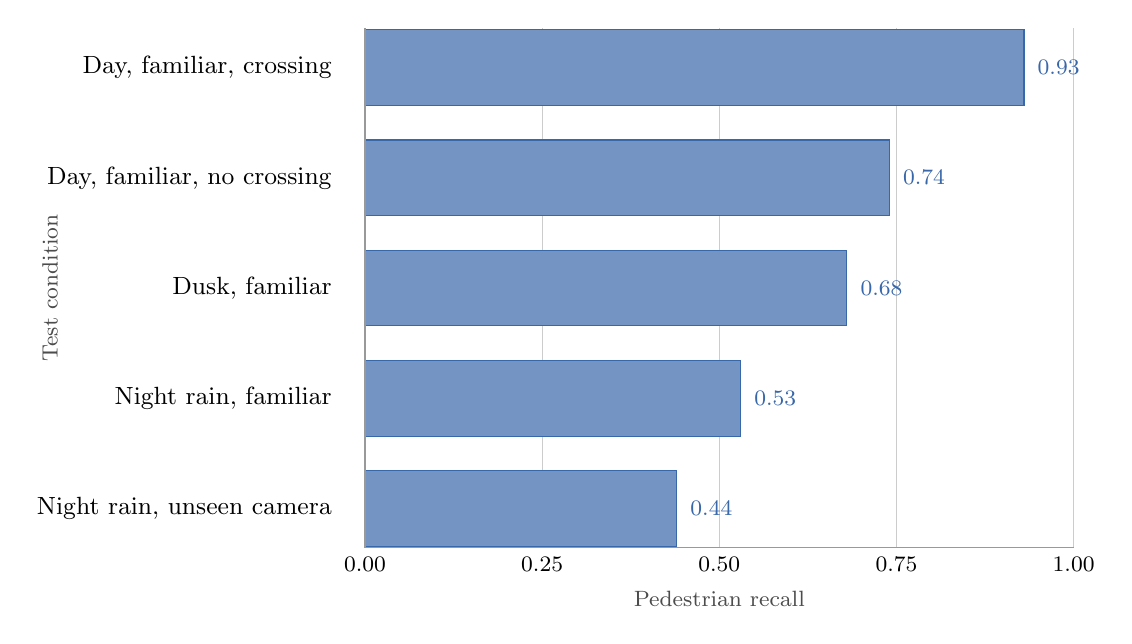
\begin{tikzpicture}[x=1cm, y=1cm, font=\small]
%% Layout: bars span x=0..9  (9cm = recall 1.0)
%%         row labels anchor=east at x=-0.3
%%         y-axis title at x=-4.2, rotated 90
%%         rows at y=0,-1.4,-2.8,-4.2,-5.6

%% ── Grid lines and x-axis ticks ──────────────────────────────────────────
\foreach \v/\lbl in {0/0.00, 2.25/0.25, 4.5/0.50, 6.75/0.75, 9.0/1.00} {
  \draw[black!20, thin] (\v, 0.5) -- (\v, -6.1);
  \node[below, font=\footnotesize] at (\v,-6.1) {\lbl};
}
%% x-axis label
\node[font=\footnotesize, black!70] at (4.5,-6.75) {Pedestrian recall};

%% ── Y-axis label (far left, clear of row labels) ─────────────────────────
\node[rotate=90, font=\footnotesize, black!70] at (-4.0,-2.8) {Test condition};

%% ── Bars (recall × 9cm) ──────────────────────────────────────────────────
%% recall values: 0.93, 0.74, 0.68, 0.53, 0.44
\def\bh{0.48}  %% half-height of each bar

\node[anchor=east, font=\small] at (-0.3, 0.0) {Day, familiar, crossing};
\fill[c8barBg]  (0,-\bh) rectangle (8.37, \bh);
\fill[c8barBlue!70] (0,-\bh) rectangle (8.37, \bh);
\draw[c8barBlue] (0,-\bh) rectangle (8.37, \bh);
\node[anchor=west, font=\footnotesize, c8barBlue] at (8.42, 0.0) {0.93};

\node[anchor=east, font=\small] at (-0.3,-1.4) {Day, familiar, no crossing};
\fill[c8barBlue!70] (0,-1.4-\bh) rectangle (6.66,-1.4+\bh);
\draw[c8barBlue] (0,-1.4-\bh) rectangle (6.66,-1.4+\bh);
\node[anchor=west, font=\footnotesize, c8barBlue] at (6.71,-1.4) {0.74};

\node[anchor=east, font=\small] at (-0.3,-2.8) {Dusk, familiar};
\fill[c8barBlue!70] (0,-2.8-\bh) rectangle (6.12,-2.8+\bh);
\draw[c8barBlue] (0,-2.8-\bh) rectangle (6.12,-2.8+\bh);
\node[anchor=west, font=\footnotesize, c8barBlue] at (6.17,-2.8) {0.68};

\node[anchor=east, font=\small] at (-0.3,-4.2) {Night rain, familiar};
\fill[c8barBlue!70] (0,-4.2-\bh) rectangle (4.77,-4.2+\bh);
\draw[c8barBlue] (0,-4.2-\bh) rectangle (4.77,-4.2+\bh);
\node[anchor=west, font=\footnotesize, c8barBlue] at (4.82,-4.2) {0.53};

\node[anchor=east, font=\small] at (-0.3,-5.6) {Night rain, unseen camera};
\fill[c8barBlue!70] (0,-5.6-\bh) rectangle (3.96,-5.6+\bh);
\draw[c8barBlue] (0,-5.6-\bh) rectangle (3.96,-5.6+\bh);
\node[anchor=west, font=\footnotesize, c8barBlue] at (4.01,-5.6) {0.44};

%% ── Axis border ──────────────────────────────────────────────────────────
\draw[black!40] (0,0.5) -- (0,-6.1);
\draw[black!40] (0,-6.1) -- (9.0,-6.1);
\end{tikzpicture}%
}
\caption{The slice pattern becomes visually obvious once recall is plotted by condition. Performance stays high in the familiar crossing regime, then falls as the detector loses crossing paint, daylight, and finally the familiar camera itself.}
\label{fig:vision-shortcut-slices}
\end{figure}

The overall benchmark score may still look respectable, especially if the test distribution resembles the daytime training distribution. Table~\ref{tab:vision-slice-breakdown} tells a different story. The detector loses much more performance when crossing markings disappear, illumination worsens, and the camera changes. Because several factors move together, the table does not identify the cause. It does support a shortcut hypothesis: background or acquisition cues may be carrying part of the signal instead of robust pedestrian evidence.

The right claim is therefore neither ``the model fails everywhere'' nor ``crossing paint is definitely the cause.'' It is narrower and more useful: the detector appears competent on the familiar camera-and-crossing regime but is not yet reliable across the deployment conditions that matter. That claim leads to better next steps---collecting non-crossing positives, holding out camera sources by design, and reviewing night failures frame by frame---rather than celebrating one aggregate score.

\begin{practicalnote}
Shortcut diagnosis usually comes from slice design, source breakdowns, and failure review---not from one dramatic heatmap. If a visual concept matters, evaluate it under the backgrounds, cameras, and conditions that might tempt the model to use something easier.
\end{practicalnote}

\subsection{Robustness and Domain Shift}

A stronger backbone improves representational power but does not guarantee that the model is using the intended evidence. An image model can perform well on the benchmark distribution and still fail under new lighting, small geometric shifts, blur or motion artifacts, different cameras or sensors, new backgrounds, or rare subgroups and unusual poses.

Average test accuracy is therefore only one part of evaluation. Vision systems should also be stress-tested under plausible shifts and broken down by subgroup, condition, and source.

\begin{evidencebox}
Evidence that a vision model is genuinely learning the intended concept should include more than clean benchmark accuracy. Useful supporting evidence includes robustness to small shifts, reasonable behavior under augmentation, inspection of failure cases, subgroup analysis, source breakdowns, and comparisons against simpler baselines.
\end{evidencebox}

\subsection{Annotation Policy and Label Noise}

Vision labels are often less objective than they first appear. For pedestrian detection, the dataset policy must decide how to label tiny far-away people, heavily occluded people, reflections, partial bodies, and cases where the person is visible but not clearly localizable. Annotation disagreement is not always a sign of bad labeling; sometimes the task boundary itself is fuzzy.

\begin{warningbox}
Write down the annotation policy before training. In vision, label noise often comes from ambiguous visibility rules, crop choices, or object-boundary disagreement rather than from random mistakes.
\end{warningbox}

\section{Robustness by Nuisance-Factor Stress Tests}

This section converts shortcut suspicion into a test plan. Organize robustness evaluation around nuisance factors: input properties that should not change the correct label but that vary across deployment conditions. Naming the factors first makes the stress tests concrete and the coverage gaps visible.

\textbf{Naming the nuisance.} For the pedestrian-detector case, the relevant nuisance factors include lighting level (daylight, dusk, night, artificial illumination), weather and precipitation (dry, wet, fog, rain on the windshield), motion blur (from the vehicle or the pedestrian), camera-specific artifacts (compression, rolling shutter, chromatic aberration), and distance-related scale change. For a medical imaging classifier, the nuisance factors include scanner model, acquisition protocol, patient position, image compression, and contrast agent.

\textbf{Predicting the failure.} Before running any test, state which nuisance factors are likely to degrade performance and why. At night, the model may rely on high-contrast edges that vanish in low light. With rain on the windshield, texture-based features may be disrupted. Making the prediction explicit before testing means the results carry information either way: a predicted failure that materializes confirms the concern; a predicted failure that does not materialize is evidence of genuine robustness.

\textbf{Testing deliberately.} Collect or synthesize examples that represent each nuisance factor at several intensity levels. Report per-nuisance performance separately, not only as an aggregate. An average that combines strong daylight performance with severe night failure hides the operational risk.

\textbf{Deciding whether the failure matters.} Not every nuisance failure requires a fix. If the deployment context excludes nighttime operation---the shuttle only runs during daylight hours---then night failure is not an operational concern. Tie the stress-test output back to the deployment specification rather than treating it as a standalone robustness ranking.

\begin{table}[t]
\centering
\small
\setlength{\tabcolsep}{4pt}
\begin{tabular}{p{2.29cm}p{2.46cm}p{2.46cm}p{2.46cm}}
\toprule
Nuisance factor & Predicted failure mode & Test method & Deploy risk? \\
\midrule
Night / low light & Misses pedestrians at distance & Held-out night clips & Yes, if shuttle runs at night \\
Rain on windshield & Spurious edge detections & Synthetic blur or real rain clips & Moderate \\
Unfamiliar campus zone & Background shortcut does not transfer & Out-of-area held-out set & Yes, if routes expand \\
\bottomrule
\end{tabular}
\caption{A structured stress-test record connects each nuisance factor to a predicted failure, a test, and a deployment-risk judgment. This prevents robustness tests from being disconnected from the deployment specification.}
\label{tab:robustness-stress-test}
\end{table}

\begin{thinkingtool}
\textbf{Nuisance-factor stress-test habit.} Name the nuisance, predict the failure, test deliberately, report per-nuisance, and judge relevance to deployment. The habit is the structure; the specific tests will differ across domains.
\end{thinkingtool}

\section{Deployment-Camera Realism}

Many of the chapter's earlier concerns collapse into one practical rule: the sensor is part of the task. Vision systems inherit the acquisition process. If benchmark images come from one camera and deployment images come from another, the task has changed even if the object categories have not. Camera height changes object geometry. Lens choice changes distortion. Compression changes texture. Exposure changes what is visible at night. Dirt, rain, glare, and rolling shutter all affect the evidence the model receives.

For the pedestrian-detector case, a training set collected from public road datasets is still an imperfect proxy for the actual shuttle camera. The shuttle may sit lower, use a wider lens, record at a different frame rate, and see more campus-specific lighting and pedestrian behavior. A system that looks strong on benchmark road scenes can still be weak on the real sensor pipeline.

\begin{decisionbox}
In vision, the deployment camera is part of the task definition. If camera geometry, image quality, or capture conditions differ materially from training, the model has not yet been tested on the real problem.
\end{decisionbox}

Before claiming the detector is ready, a minimal stress-test matrix should at least cover daylight, dusk, and night; dry roads, rain, and glare; familiar and unseen camera sources; marked crossings and unmarked curb approaches; and near, medium, and far pedestrian scale.

This is not bureaucratic caution. It is how the team learns whether the system is robust to the actual image-acquisition process or only to the benchmark story.

\section{Saliency Is Diagnostic Evidence, Not Proof}

Students sometimes hope a heatmap or saliency map fully explains a model. Such tools can be informative but are not definitive. Explanation methods are themselves model-dependent and can be unstable. Treat them as diagnostic evidence, not as proof that the model ``looked at the right thing.''

This matters because the rest of the chapter is about evidence quality. A saliency map may localize suspicion or hint at model focus, but it cannot by itself settle whether the model learned the intended cue or a shortcut.

\begin{example}[Saliency Suggests, Stress Tests Decide]
A saliency map for a pedestrian detector might highlight bright crosswalk paint near a person. That is a useful suspicion, not a verdict. Stronger evidence would occlude the paint, compare marked and unmarked crossings, test camera-source holdouts, and inspect low-light or rainy slices. If performance collapses only when the crosswalk cue disappears, the shortcut hypothesis becomes much stronger than any heatmap alone could make it.
\end{example}

\section{Chapter Artifact: A Vision Design and Stress-Test Card}

By the end of this chapter, you should be able to produce a one-page design and stress-test card before making a serious vision claim. The framing memo named the decision, the metric worksheet named good behavior, the evaluation plan protected the claim, the baseline sheet justified linearity, the structure diagnosis sheet justified leaving it, the training report justified the learned-model claim, and the reuse-and-adaptation plan clarified what transfer could legitimately explain. This card adds the vision-specific layer: what the camera sees, what variation should be ignored, what shortcuts are likely, and what slices must be passed before a benchmark result means anything operational.

\begin{table}[t]
\centering
\small
\setlength{\tabcolsep}{4pt}
\begin{tabular}{p{3.25cm}p{6.98cm}}
\toprule
Card field & What must be written clearly \\
\midrule
Seven-question focus & Questions 3, 4, 6, and 7: what image evidence exists, what visual structure matters, what tests justify the claim, and how deployment conditions affect action \\
Task type & Classification, detection, segmentation, tracking, or another structured vision output \\
Target visual signal & What visual content the model is truly supposed to use \\
Nuisance variations to ignore & Lighting, small translation, blur, background, viewpoint, or other variations that should preserve the label \\
Variations that should change the label & The changes that really do alter the class or output structure \\
Acceptable augmentations & Which label-preserving transformations are justified by the task \\
Likely shortcut risks & Background, watermark, scanner marker, room lighting, crop policy, or sensor artifact \\
Pretrained backbone choice & What representation source will be reused and why \\
Deployment camera or sensor & What image-acquisition process the real system will actually face \\
Critical slices & Which deployment-relevant conditions such as night, rain, unseen cameras, rare poses, or changed backgrounds must be checked separately \\
Required stress tests & Shift tests, subgroup checks, source breakdowns, or robustness probes that must be run before a claim is trusted \\
\bottomrule
\end{tabular}
\caption{A vision design and stress-test card turns the chapter's ideas into a practical protocol before benchmark numbers are reported.}
\label{tab:vision-stresstest-card}
\end{table}

\begin{thinkingtool}
\textbf{Vision design and stress-test card.} Before reporting performance, write down the task type, intended signal, nuisance variation, acceptable augmentations, shortcut risks, deployment camera, critical slices, and required stress tests.
\end{thinkingtool}

\begin{example}[Filled Vision Design Card]
For a pedestrian detector on dashboard-camera footage, a sensible card reads as follows. Task type: \emph{detection}. Target visual signal: pedestrian shape, motion, and local road context. Nuisance variations: small translation, daylight change, and mild blur. Label-changing variations: replacing the pedestrian with a sign or removing the pedestrian entirely. Acceptable augmentations: small crops, brightness changes, and mild weather corruption---but not vertical flips or unrealistic rotations. Shortcut risks: crossing paint, road background, camera height, and annotation crop policy. Backbone: a pretrained road-scene detector. Deployment: a low-mounted dashboard camera at dusk and night as well as daytime. Critical slices: marked versus unmarked crossings, night rain, and unseen camera sources. Required stress tests: low-light slices, rain, glare, source-heldout evaluation, and manual review of missed close-range pedestrians.
\end{example}

\section{Common Mistakes in Vision}

The recurring mistakes in vision are failures to connect pixel measurements back to the real task. Readers treat pixels as independent features even when locality and neighborhood structure are central, apply augmentations without asking what they mean in the world, declare understanding from benchmark accuracy alone, ignore data-collection bias, and forget that the deployment camera and acquisition process are part of the problem rather than neutral background details.

\section{Looking Ahead}

This chapter grounded representation learning in vision: invariance, locality, augmentation, shortcut learning, and camera realism. The next chapter keeps the same methodological discipline but changes the source of difficulty. Instead of asking which visual variation should be ignored, it asks which linguistic context must be preserved---and when external grounding is needed before fluent output can be trusted.

\section*{Chapter Summary}

This chapter treated vision as a problem of preserved and discarded variation. Task formulation, annotation policy, convolutional structure, augmentation, and robustness testing are all ways of deciding which visual changes should and should not matter. The central lesson is that benchmark success is not enough: a credible vision system must show that it learned the intended signal and that this signal survives the lighting, camera, and scene changes that deployment will actually produce.

\begin{studyquestions}
\item Why is it misleading to think of image understanding as only a pixel-processing problem?
\item What does an invariance audit force the modeler to state explicitly?
\item What does parameter sharing buy us in a convolutional layer?
\item Why can max pooling make a representation less sensitive to tiny image shifts?
\item Why must augmentation choices depend on the task?
\item Why does high benchmark accuracy not prove robust visual understanding?
\item Why can a pedestrian detector look strong on familiar crossings yet still be weak on the real deployment route?
\end{studyquestions}

\begin{exercises}
\item \exercisetag{Calculation}{Core}Use the vertical-edge filter from the chapter on a new $3 \times 3$ patch of your own design. Compute the convolution response by hand.
\item \exercisetag{Concept}{Core}Explain in words why a dense network on raw pixels may need far more parameters than a convolutional network to detect the same local pattern at many image positions.
\item \exercisetag{Concept}{Core}Perform a short invariance audit for a pedestrian-detection system. Name two variations that should preserve the label and two that should change what the system must output.
\item \exercisetag{Concept}{Core}Give one example of an augmentation that is likely helpful for a generic object classifier and one example of an augmentation that could be harmful in a specialized vision task.
\item \exercisetag{Concept}{Intermediate}Describe a real-world setting in which object detection is necessary but classification alone is insufficient.
\item \exercisetag{Concept}{Intermediate}Give two examples of shortcut signals a vision model might exploit in a poorly designed dataset.
\item \exercisetag{Concept}{Intermediate}Suppose a model performs well on benchmark photos but poorly on low-light phone images from deployment. Give two plausible technical reasons for the gap.
\item \exercisetag{Design}{Intermediate}Sketch a minimal stress-test matrix for a dashboard-camera pedestrian detector. Include at least one lighting slice, one weather slice, one source slice, and one scene-structure slice.
\item \exercisetag{Design}{Intermediate}Use Table~\ref{tab:vision-stresstest-card} to sketch a one-page design and stress-test card for a vision task of your choice. If you are carrying one case through the book, explicitly preserve the same task, review policy, and evaluation commitments while adding the vision-specific invariance and shortcut checks.
\item \exercisetag{Implementation}{Core}Implement a $3\times 3$ vertical-edge filter from scratch in \verb|numpy|. Construct a $32\times 32$ synthetic grayscale image with a single vertical bar of brighter pixels and small Gaussian noise elsewhere. Apply your convolution (no \verb|scipy| or \verb|torch| call) using the kernel $\begin{pmatrix}-1 & 0 & 1\\ -1 & 0 & 1\\ -1 & 0 & 1\end{pmatrix}$, then display the input and the rectified response side by side. Verify that the response peaks near the bar's edge columns and is near zero elsewhere; rotate the bar to horizontal and confirm the response collapses, illustrating the filter's directional selectivity.
\item \exercisetag{Implementation}{Intermediate}Add a translation-invariance check on top of the previous exercise. Shift your synthetic image by 1, 4, and 8 pixels horizontally and recompute the rectified convolution map. Show that the response simply translates with the input (equivariance). Then apply $2\times 2$ max pooling with stride 2 to each map, and report by how much each shift changes the pooled feature vector measured in $\ell_2$. Comment on why pooling reduces but does not remove sensitivity to position.
\end{exercises}

\begin{challengeexercises}
\item \exercisetag{Concept}{Advanced}Explain carefully why convolution supports translation equivariance rather than perfect invariance, and why later layers or augmentation are still needed.
\item \exercisetag{Diagnosis}{Advanced}A vision model trained to detect disease from scans performs extremely well, but a hospital discovers that the model relies heavily on scanner-specific marks. Explain how this can happen and propose an evaluation protocol that would reveal it.
\item \exercisetag{Diagnosis}{Advanced}Compare two deployment strategies for a small vision dataset: frozen pretrained backbone plus linear head, versus full fine-tuning. State when each would be preferable and what evidence would justify the choice.
\item \exercisetag{Diagnosis}{Advanced}A vision design card proposes vertical flips, large rotations, and heavy color stylization for a fixed dashboard-camera pedestrian detector. Mark which invariance claims are unjustified, which deployment slices should be tested, and what augmentation policy would be safer.
\item \exercisetag{Design}{Advanced}Design a stress-test suite for a road-scene pedestrian detector that uses at least four shift types or subgroup checks. Explain what failure in each case would mean.
\end{challengeexercises}
